\documentclass[11pt,letterpaper]{article}

\newenvironment{proof}{\noindent{\bf Proof:}}{\qed\bigskip}

\newtheorem{theorem}{Theorem}
\newtheorem{corollary}{Corollary}
\newtheorem{lemma}{Lemma} 
\newtheorem{claim}{Claim}
\newtheorem{fact}{Fact}
\newtheorem{definition}{Definition}
\newtheorem{assumption}{Assumption}
\newtheorem{observation}{Observation}
\newtheorem{example}{Example}
\newcommand{\qed}{\rule{7pt}{7pt}}

\newcommand{\solution}[4]{
\thispagestyle{plain} 
\newpage
\setcounter{page}{1}
\noindent
\begin{center}
\framebox{ \vbox{
\vspace{4mm}
\vspace{0.2in} 
{\centering \large\mbox{#3}}\\
\vspace{0.1in}
{#1 \hfill {Date: #2}}
}}
\end{center}
\markright{#1}
}

\newenvironment{algorithm}
{\begin{center}
\begin{tabular}{|l|}
\hline
\begin{minipage}{1in}
\begin{tabbing}
\quad\=\qquad\=\qquad\=\qquad\=\qquad\=\qquad\=\qquad\=\kill}
{\end{tabbing}
\end{minipage} \\
\hline
\end{tabular}
\end{center}}

\def\Comment#1{\textsf{\textsl{$\langle\!\langle$#1\/$\rangle\!\rangle$}}}



\usepackage{graphicx, amssymb, amsmath, listings, float, mathtools}
\usepackage{color, url}
\usepackage{caption}
\lstset{language = Python}
\lstset{breaklines}
\lstset{extendedchars=false}

\oddsidemargin 0in
\evensidemargin 0in
\textwidth 6.5in
\topmargin -0.6in
\textheight 9.0in

\begin{document}

\solution{\large Jifu Zhao}{\large 09/15/2016}{\bf \Large ECE 544NA \hspace{0.5cm} 
		Fall 2016 \hspace{0.5cm} Assignment 1}

\section*{\Large I. Pencil-and-Paper}
\begin{description}
%%%%%%%%%%%%%%%%%%%%%%%%%%%%%%%%%%%%%%%%%%%%%%%%%%%%%%%%%%%%%%%%%%%%%%%%%%%%%%%%%%%%%%%%%
% Problem 1
\item{\bf \large 1. Find the derivatives $\frac{dE}{dw_j}$ and $\frac{dE}{db}$.}

From
\begin{equation} \label{eq1}
	E = \sum_i{((t_i - y_i)^2)}
\end{equation}

\begin{equation}
\begin{split}
	\frac{dE}{dw_j} & = \frac{d(\sum_i{((t_i - y_i)^2)})}{dw_j} \\
					& = \sum_i{\frac{d(t_i - g(w' x_i + b))^2}{dw_j}} \\
					& = -2\sum_i{(t_i - g(w' x_i + b))\frac{dg(w' x_i + b)}{dw_j}} \\
					& = -2\sum_i{(t_i - g(w' x_i + b))g'(w' x_i + b) x_{ij}}
\end{split}
\end{equation}
{\bf Note: }$x_{ij}$ means the jth feature of ith element $x_i$, corresponding to $w_j$.

\begin{equation}
\begin{split}
	\frac{dE}{db} & = \frac{d(\sum_i{((t_i - y_i)^2)})}{db} \\
				  & = \sum_i{\frac{d(t_i - g(w' x_i + b))^2}{db}} \\
				  & = -2\sum_i{(t_i - g(w' x_i + b))\frac{dg(w' x_i + b)}{db}} \\
				  & = -2\sum_i{(t_i - g(w' x_i + b))g'(w' x_i + b)}
\end{split}
\end{equation}\\

%%%%%%%%%%%%%%%%%%%%%%%%%%%%%%%%%%%%%%%%%%%%%%%%%%%%%%%%%%%%%%%%%%%%%%%%%%%%%%%%%%%%%%%%%
% Problem 2
\item{\bf \large 2. Write $\frac{dE}{dw_j}$ without $g'()$.}

Since $g(a) = a$, so $g'(a) = 1$, so from part 1:

\begin{equation}
\begin{split}
	\frac{dE}{dw_j} & = -2\sum_i{(t_i - g(w' x_i + b))g'(w' x_i + b) x_{ij}} \\
					& = -2\sum_i{(t_i - (w' x_i + b)) x_{ij}} \\
\end{split}
\end{equation}\\

%%%%%%%%%%%%%%%%%%%%%%%%%%%%%%%%%%%%%%%%%%%%%%%%%%%%%%%%%%%%%%%%%%%%%%%%%%%%%%%%%%%%%%%%%
% Problem 3
\item{\bf \large 3. Write $g'(w' x_i + b)$ when $g(a) = \frac{1}{1 + exp(-a)}$.}
\begin{equation}
\begin{split}
	g'(a) & = \frac{exp(-a)}{(1 + exp(-1))^2} \\
		  & = \frac{1}{1 + exp(-a)} \frac{exp(-a)}{1 + exp(-a)} \\
		  & = \frac{1}{1 + exp(-a)} (1 - \frac{1}{1 + exp(-a)}) \\
		  & = g(a) (1 - g(a))
\end{split}
\end{equation}
In this way,
\begin{equation}
	g'(w' x_i + b) = y_i (1 - y_i)
\end{equation}

\begin{equation}
	\frac{dE}{dw_j} = -2\sum_i{(t_i - y_i) y_i (1 - y_i) x_{ij}}
\end{equation}

\begin{equation}
	\frac{dE}{db} = -2\sum_i{(t_i - y_i) y_i (1 - y_i)}
\end{equation}\\

%%%%%%%%%%%%%%%%%%%%%%%%%%%%%%%%%%%%%%%%%%%%%%%%%%%%%%%%%%%%%%%%%%%%%%%%%%%%%%%%%%%%%%%%%
% Problem 4
\item{\bf \large 4. Use the perceptron error: $E = \sum_i{(max(0, -(w' x_i + b) \cdot t_i))}$.}

When $E = \sum_i{(max(0, -(w' x_i + b) \cdot t_i))}$, suppose we have:
\begin{equation}
E = \sum_{i: t_i \neq sign(w' x_i + b)}{(-(w' x_i + b) \cdot t_i)}
\end{equation}
Then, we can can calculate:

\begin{equation}
\begin{split}
	\frac{dE}{dw_j} & = \frac{d\sum_i{(max(0, -(w' x_i + b) \cdot t_i))}}{dw_j} \\
					& = \sum_{i: t_i \neq sign(w' x_i + b)}{\frac{d(-(w' x_i + b) \cdot t_i)}{dw_j}} \\
					& = \sum_{i: t_i \neq sign(w' x_i + b)}{-x_{ij} \cdot t_i}
\end{split}
\end{equation}
In the same way, 
\begin{equation}
\begin{split}
	\frac{dE}{db} & = \frac{d \sum_i{(max(0, -(w' x_i + b) \cdot t_i))}}{db} \\
			      & = \sum_{i: t_i \neq sign(w' x_i + b)}{\frac{d(-(w' x_i + b) \cdot t_i)}{b}} \\
				  & = \sum_{i: t_i \neq sign(w' x_i + b)}{-t_i}
\end{split}
\end{equation}\\

%%%%%%%%%%%%%%%%%%%%%%%%%%%%%%%%%%%%%%%%%%%%%%%%%%%%%%%%%%%%%%%%%%%%%%%%%%%%%%%%%%%%%%%%%
% Problem 5
\item{\bf \large 5. Use the SVM error: $E = ||w||^2_2 + C \cdot \sum_i{(h(x_i, t_i))}$, where 
	  $h(x_i, t_i) = max(0, 1 - t_i (w' x_i + b))$.}
	  
In this case, since $E = ||w||^2_2 + C \cdot \sum_i{(h(x_i, t_i))}$, 
where $h(x_i, t_i) = max(0, 1 - t_i (w' x_i + b))$, we can simplify it into:
\begin{equation}
\begin{split}
	E = \sum_k{w_k^2} + C \cdot \sum_{i: t_i(w' x_i + b) < 1}{1 - t_i(w' x_i + b)}
\end{split}
\end{equation}

\begin{equation}
\begin{split}
	\frac{dE}{dw_j} = 2w_j - C \cdot \sum_{i: t_i(w' x_i + b) < 1}{x_{ij} \cdot t_i}
\end{split}
\end{equation}
\begin{equation}
\begin{split}
	\frac{dE}{db} = - C \cdot \sum_{i: t_i(w' x_i + b) < 1}{t_i}
\end{split}
\end{equation}\\
\end{description}


\newpage
\section*{\Large II. Code-from-Scratch}

\subsection*{\large 1. Methods}
In this section, two helper function are defined: $readFile(labelPath, featureDir)$ and $addBias(data)$. And two classes named $GDclassifier(object)$ and $PCA(object)$ are the main parts for this assignment. The dependency of the functions is shown in Figure \ref{fig:diagram}

\begin{figure}[H]
\centering
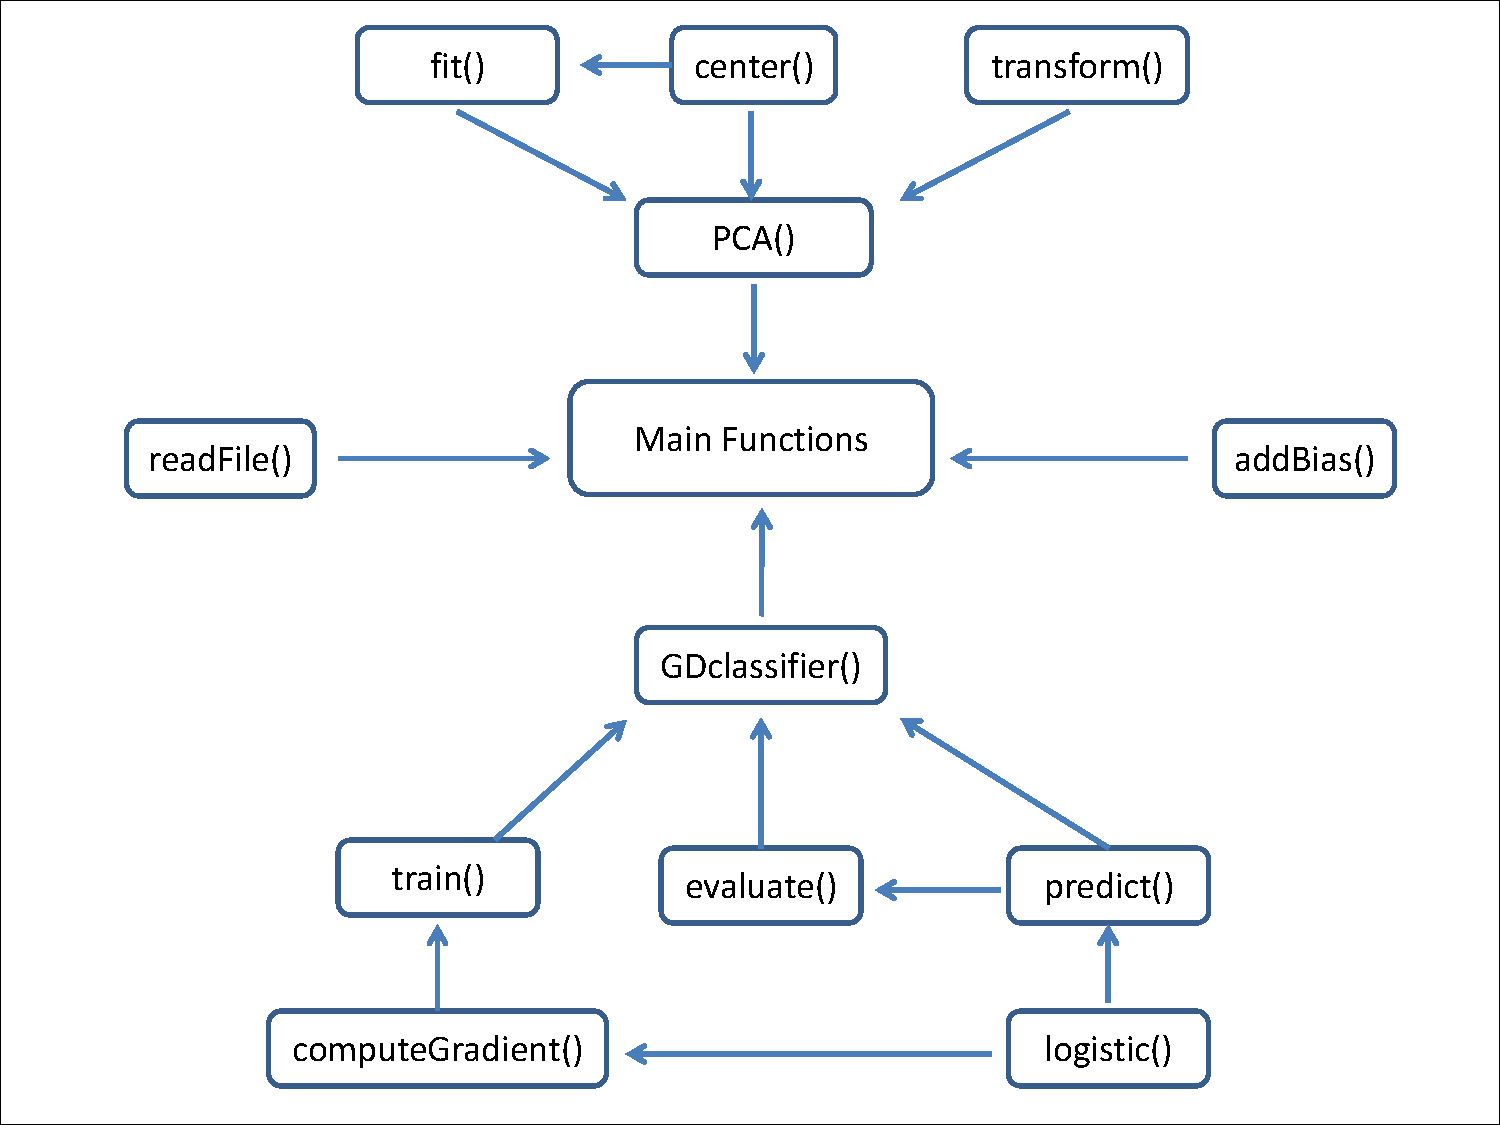
\includegraphics[width=0.8\textwidth]{./figures/diagram.pdf}
%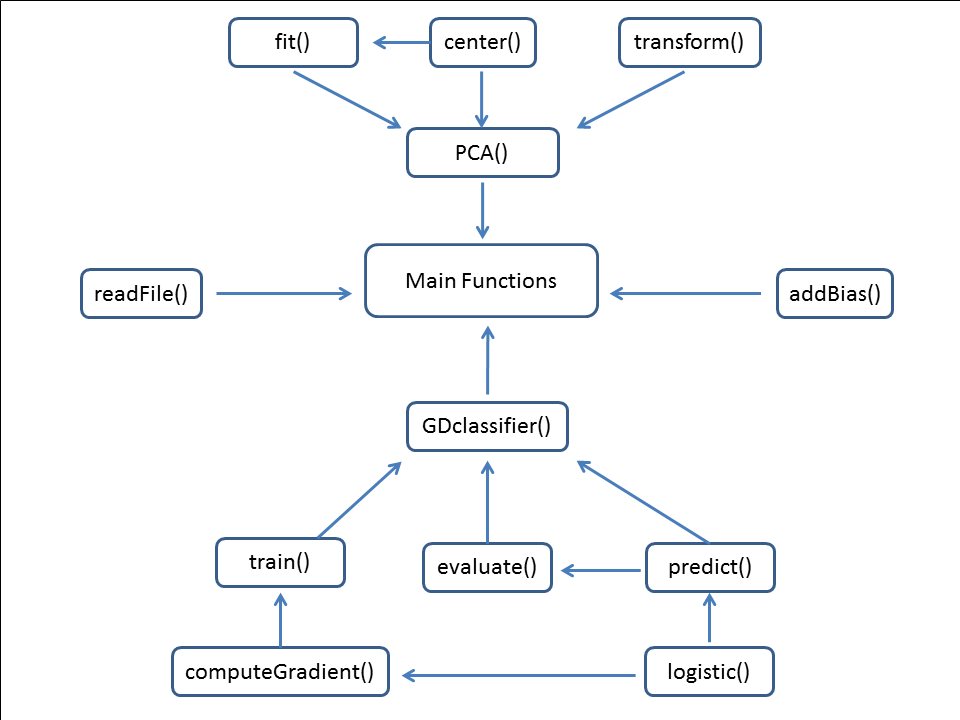
\includegraphics[width=0.9\textwidth]{./figures/diagram.png}
\caption{\label{fig:diagram} Function Dependency Diagram}
\end{figure}

\begin{description}
\item[Function: ] $\bf readFile(labelPath, featureDir)$\\ 
	Function $readFile()$ is going to read the data from the specified path. It returns two numpy.array: $features$ and $labels$. The $features$ array has dimension $n \times m$, where n is the number of data and m is the number of features. The $labels$ array has dimension $n \times 1$, corresponding to the labels for each input. 
	
\item[Function: ] $\bf addBias(data)$\\ 
	Function $addBias(data)$ is used to add bias 1 to each row in data. For example, if the input data has dimension $n \times m$, then this function will add 1 to each row as the first column and return a matrix with dimension $n \times (m + 1)$ 
	
\item[Class: ] $\bf GDclassifier(object)$\\ 
	Class $GDclassifier(object)$ is the implementation of Gradient Descent methods to train four classifiers: linear, logistic, perceptron, and linear SVM. It has several parts.
	
	\begin{description}
		
	\item $\bf train(self, X, y)$\\
		Function to train the model. It use the gradient descent method, where 
		\begin{equation}
			w_t = w_{t-1} - \eta \cdot \frac{dE}{dw} / n
		\end{equation}
		Note that in the above equation, $\eta$ is the learning rate and to make sure that the gradient descent is not too large, $\frac{dE}{dw}$ is divided by the input numbers $n$.
		
	\item $\bf predict(self, X, w)$\\
		Function $predict(self, X, w)$ is used to get the prediction for input X.
	
	\item $\bf evaluate(self, X, y, w)$\\
		Function $evaluate(self, X, y, w)$ is used to calculate the Error and accuracy for given X, y and w.
	
	\item $\bf computeGradient(self, X, y, w)$\\
		Function $computeGradient(self, X, y, w)$ is used to calculate the gradient descent $\frac{dE}{dw}$. 
		(a) When loss='linear', it calculates according Equation (4), which corresponds to line 124 in codes.\\
		(b) When loss='logistic', it calculates according Equation (7) and (8), which corresponds to line 126 in codes.\\
		(c) When loss='perceptron', it calculates according Equation (10) and (11), which corresponds to line 129 in codes.\\
		(d) When loss='svm', it calculates according Equation (13) and (14), which corresponds to line 135 in codes.
	
	\item $\bf logistic(self, X, w)$\\
		Function $logistic(self, X, w)$ is used to calculate the logistic function. It returns 
		$$g(x_i) = \frac{1}{1 + exp(- w' x_i)}$$
	
%	\item $\bf getParams(self)$\\
%		Function $getParams(self)$ is used to get the recorded training MSE, training accuracy and w.
%
%	\item $\bf plot(self, figsize=(12, 5))$\\
%		Function $plot(self, figsize=(12, 5))$ is a helper function to plot the change of training MSE and training accuracy vs. iterations.
	\end{description}

\item[Class: ] $\bf PCA(object)$ \\
	Class $PCA(object)$ is the implementation of Principal Component Analysis for the given data. It has following three main parts.
	\begin{description}
	\item $\bf fit(self, X)$ \\
		Function $fit(self, X)$ uses function $center(self, X)$ to calculate the mean value for each dimension, and then through SVD, calculate the eigenvector and corresponding variance.
	
	\item $\bf center(self, X)$ \\
		Function $center(self, X)$ calculate the mean value for each dimension.
	
	\item $\bf transform(self, X)$ \\
		Function $transform(self, X)$ project the given X onto designated principal components. Note, it will not center the data first, so you may need to manually center the data first.
	
	\end{description}

\end{description}

\newpage
\subsection*{\large 2. Results}
\noindent {\bf Part a.}\\

For linear, logistic, perceptron and linear SVM classifier, through training classifier on the training set and choosing appropriate learning rate through development set, the final convergence plots of error rate for four classifiers are shown in Figure \ref{fig:convergence}.

\begin{figure}[H]
\centering
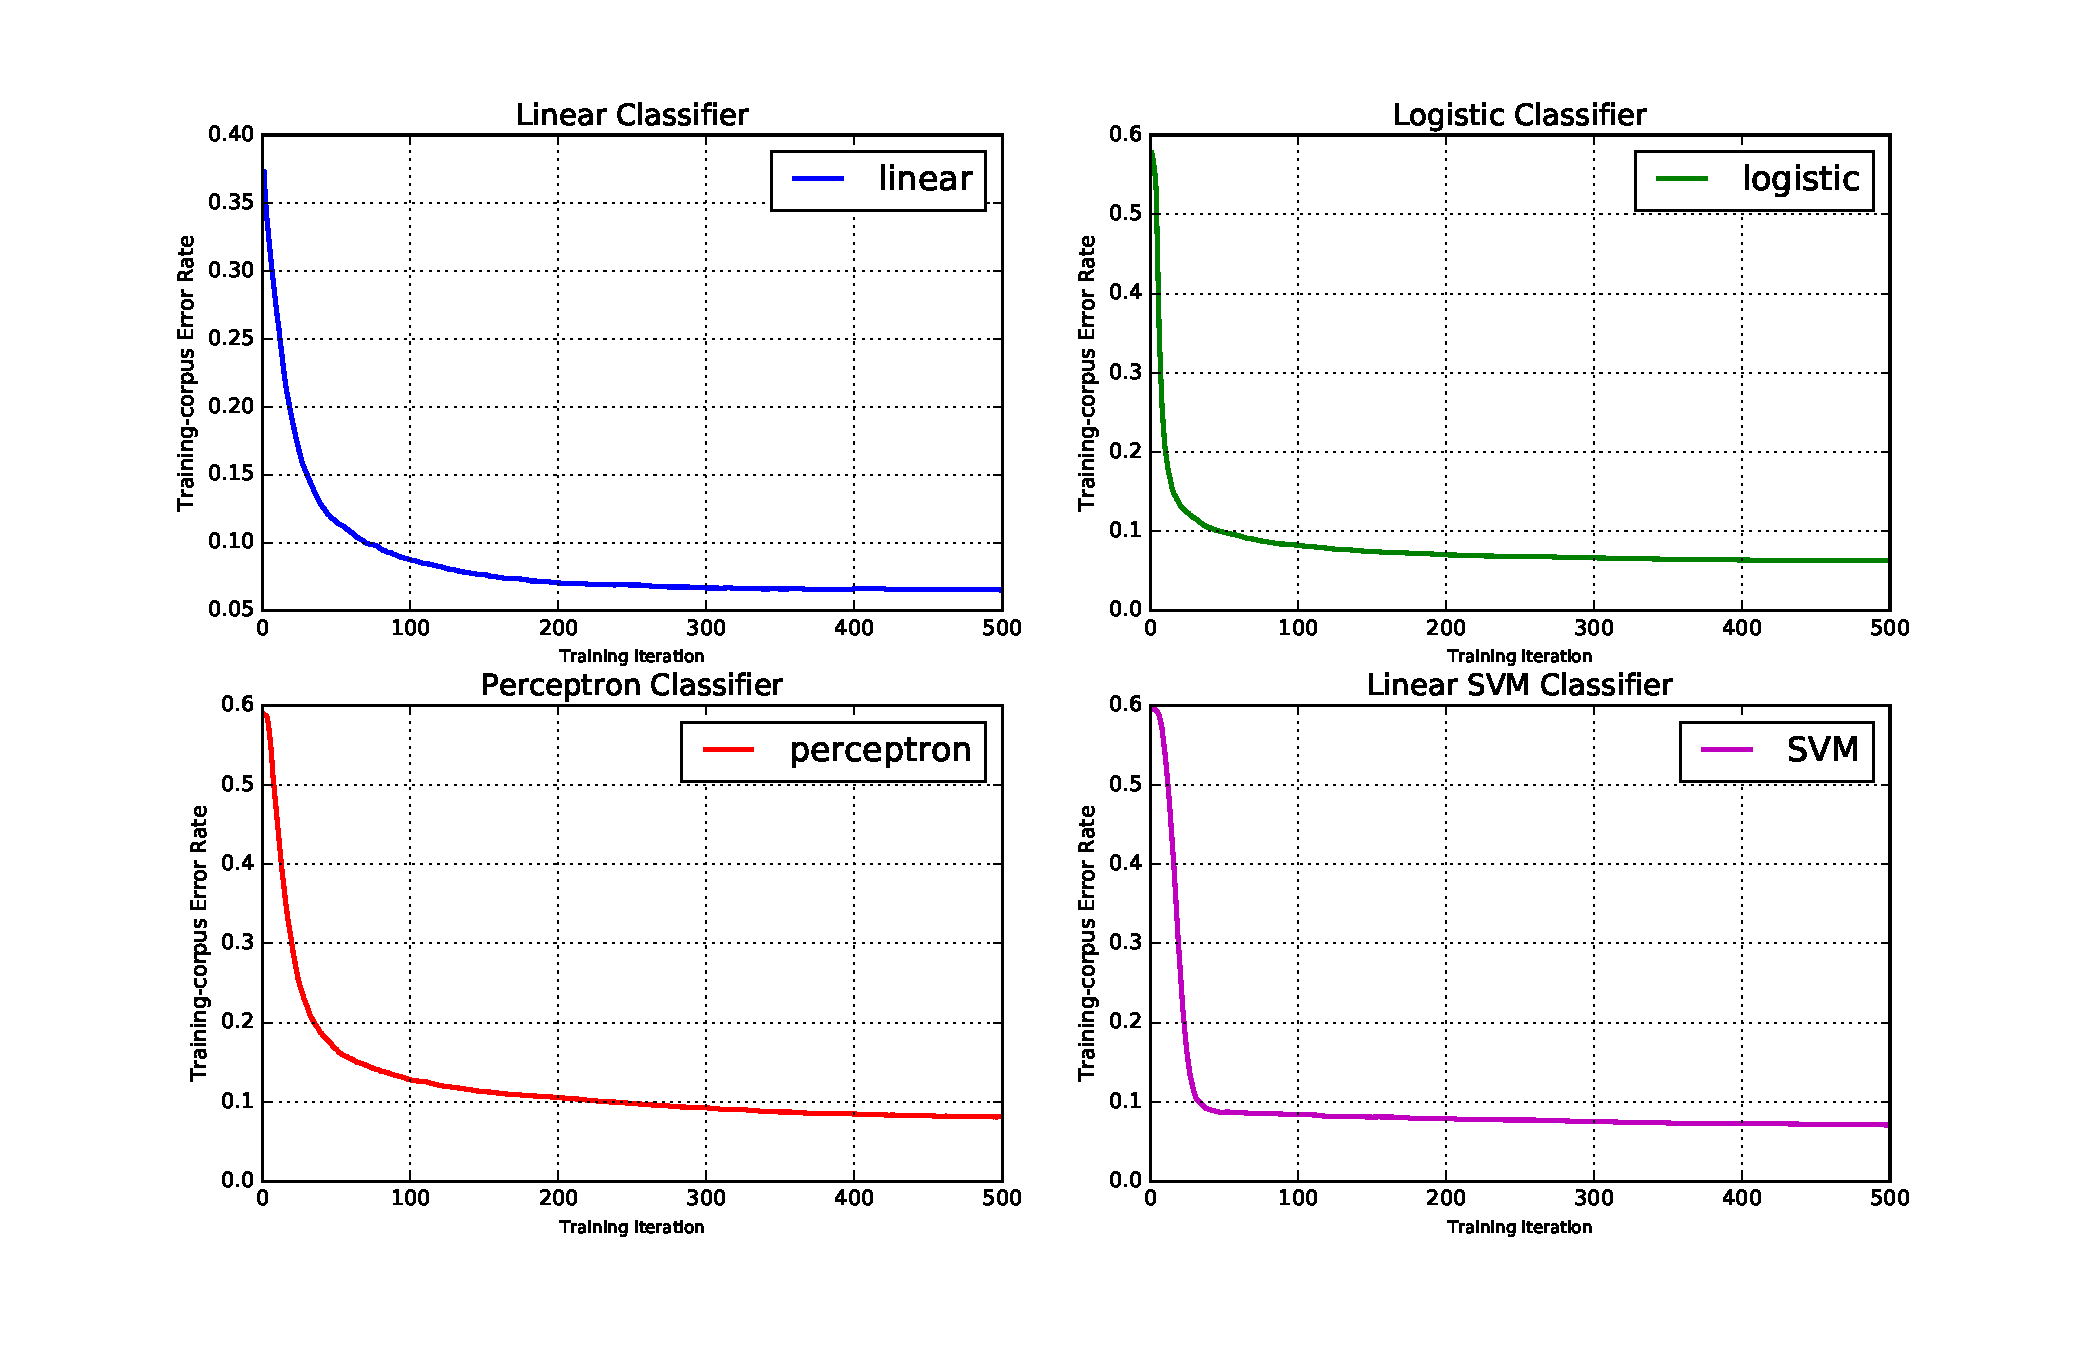
\includegraphics[width=1.0\textwidth]{./figures/covergence.pdf}\
\caption{\label{fig:convergence} Training corpus error rate convergence curve}
\end{figure}

In Figure \ref{fig:convergence}, the learning rate are 0.01, 0.5, 0.05, 0.01 for linear, logistic, perceptron and linear SVM classifier respectively, and C is chosen to be 1 for SVM classifier. All these four algorithms use 500 iterations.\\

\noindent {\bf Part b.}\\

In this part, using the training corpus as the training set and development corpus as the validation set, through choosing different values of C and the best learning rate, the corresponding error rate for training corpus and development corpus are shown in Figure \ref{fig:svm}.

\begin{figure}[H]
\centering
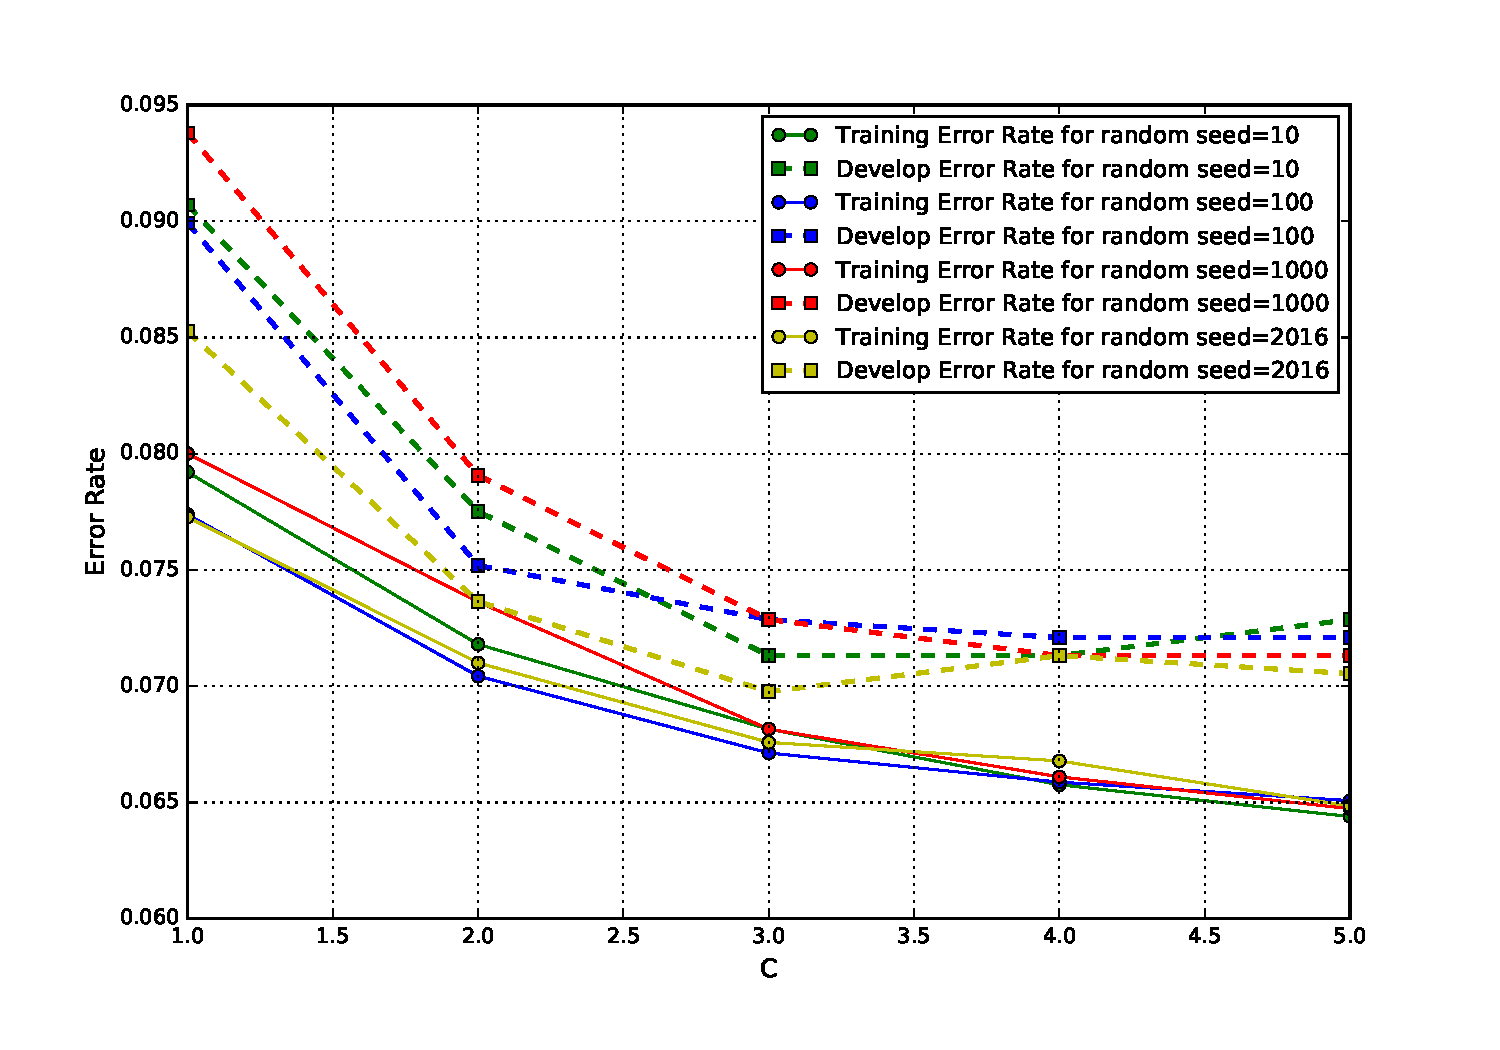
\includegraphics[width=1.0\textwidth]{./figures/svm-comparison.pdf}
%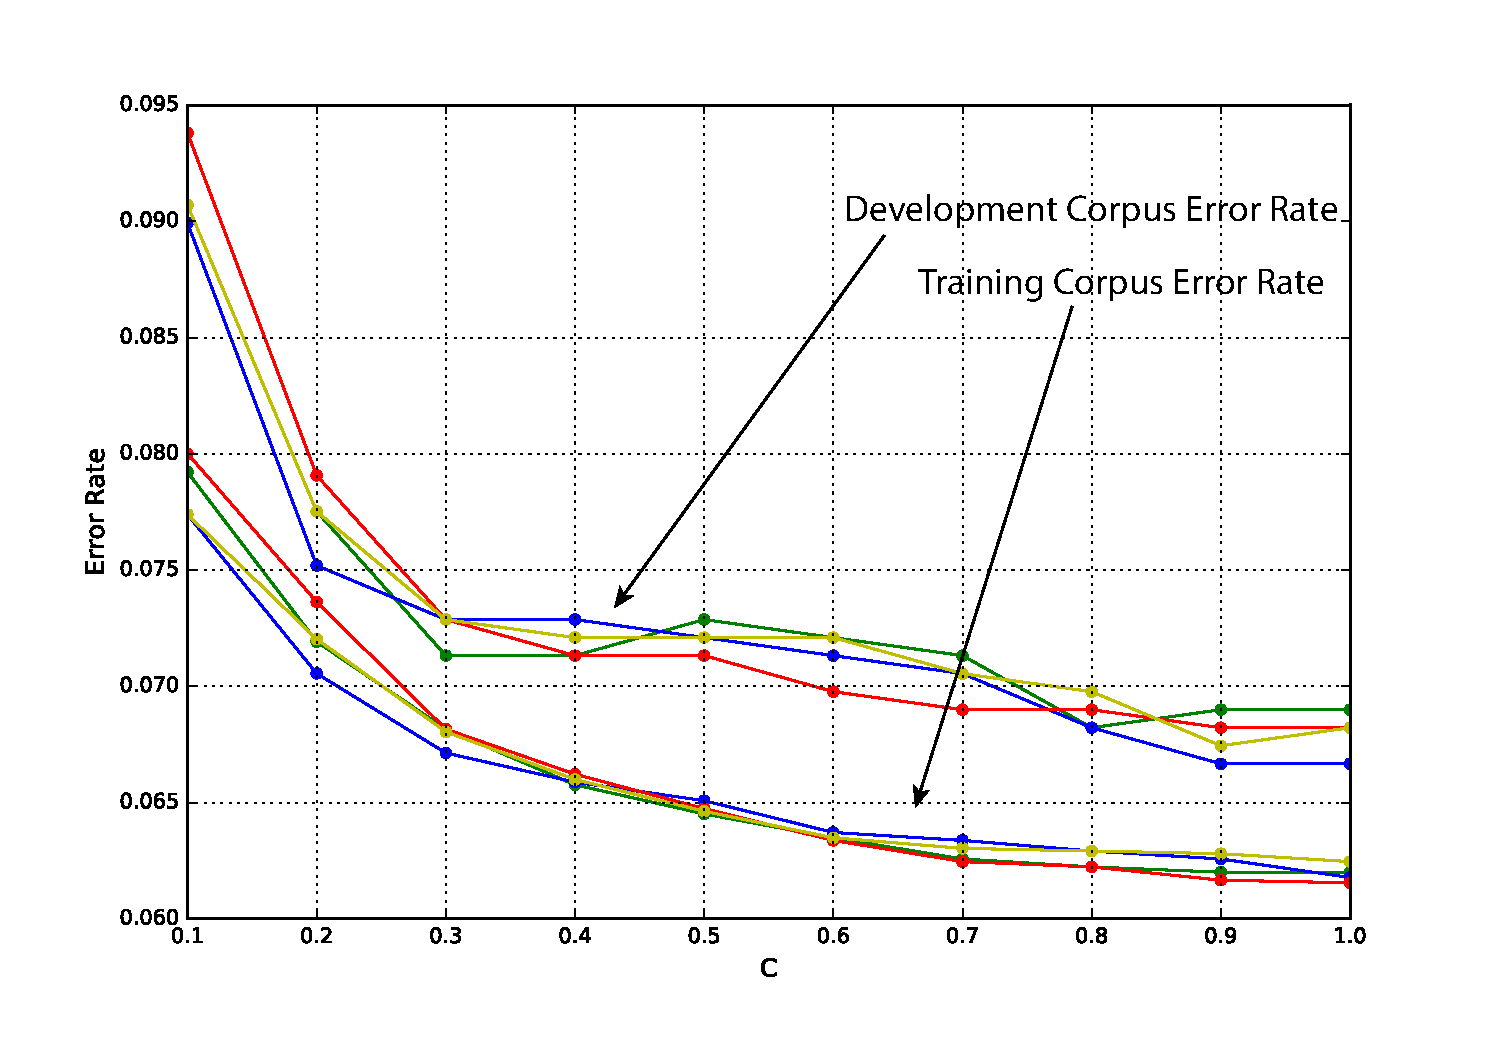
\includegraphics[width=1.0\textwidth]{./figures/svm-comparison3.pdf}
\caption{\label{fig:svm} SVM error rate comparison}
\end{figure}

In Figure \ref{fig:svm}, the values of C are setting to be 1.0, 2.0, 3.0, 4.0 and 5.0, and the learning rate is fixed to be 0.005. Through using different random seed: 10, 100, 1000 and 2016, we can have different random initialization for w and b. In this way, each C has 4 corresponding training corpus error rate and 4 corresponding development corpus error rate. The details are shown in Figure \ref{fig:svm}.\\


\noindent {\bf Part c.}\\

In this part, using the result from Part a. and Part b., the corresponding table for evaluation test corpus error rates for all four classifiers are shown in Table \ref{table:error}.

\begin{table}[H]
	\centering
	\caption{Comparison of error rate for different classifiers}
	\label{table:error}	
	\begin{tabular}{c | c}
		\hline \hline
		Classifier  &	Error rate \\[0.1cm]
		\hline
		Linear regression		&	3.15\%	\\[0.1cm]
		Logistic regression		&	4.07\%	\\[0.1cm]
		Perceptron				&	5.37\%	\\[0.1cm]
		Linear SVM				&	3.77\%	\\[0.1cm]
		\hline	
	\end{tabular}
\end{table}

In Table \ref{table:error}, the learning rates are 0.01, 0.5, 0.05, 0.05 for linear, logistic, perceptron and linear SVM classifier respectively, and C is chosen to be 1.0 for SVM classifier.\\


\noindent {\bf Part d.}\\

In this part, the PCA is conducted based on all the training corpus, then randomly choose 300 examples without replacement. The four boundary is calculated based on the result from Part a.

\begin{figure}[H]
\centering
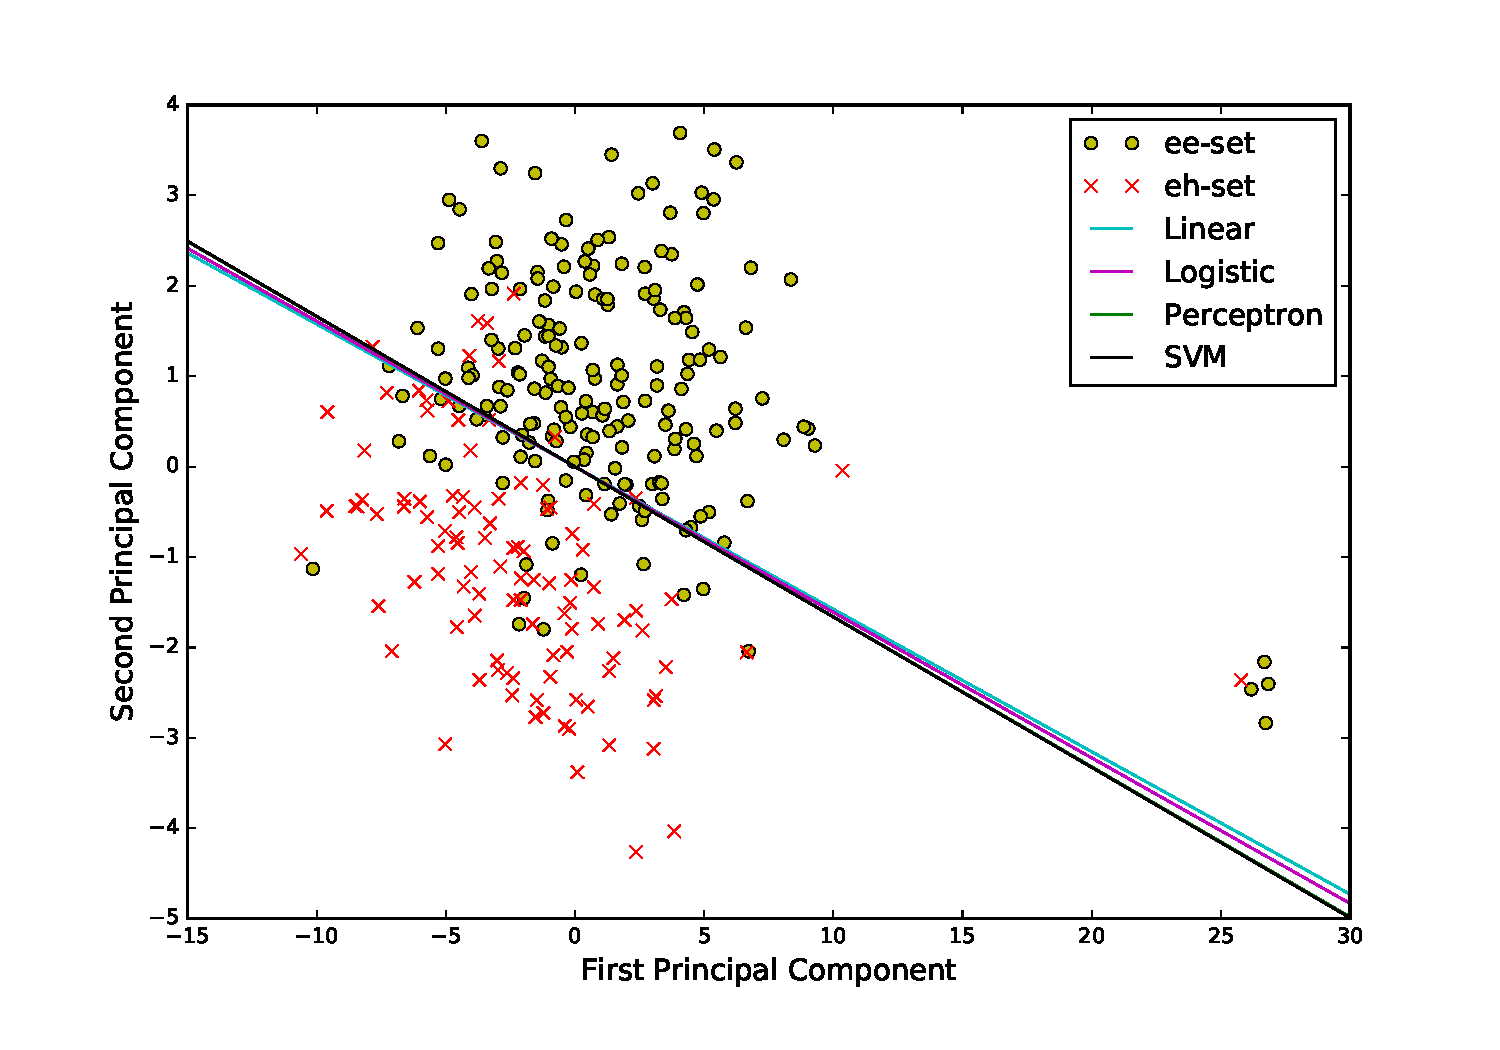
\includegraphics[width=1.0\textwidth]{./figures/PCA.pdf}
\caption{\label{fig:pca} PCA projection}
\end{figure}

Note: in Figure \ref{fig:pca}, for the selected 300 points, the first step is subtracting the mean value for each dimension. Then, project them onto the first eigenvectors calculated through PCA. And for the PCA part, all input data have been added the bias term, which is 1 for all input data.

\newpage
\section*{\Large III. TensorFlow}

\subsection*{\large 1. Methods}
In this part, we define the expression for classifier should be $y = w'x + b$, where b is a bias term. For convenience, we use One-Hot-Encoding to process the labels such that:
$$ label \ 0 := [1, 0] $$
$$ label \ 1 := [0, 1] $$
So, the output has two dimensions. To transform the output to be the probability, we use softmax function, in which:
\begin{equation}
 y = softmax(w'x + b) 
\end{equation}
where $softmax(a)_i = \frac{exp(a_i)}{\sum_j{exp(x_j)}}$

The above expression in TensorFlow is written as 
$$y = tf.nn.softmax(tf.matmul(x, W) + b)$$
For this problem, the dimension of x is $n \times 16$, the dimension of w is $16 \times 2$, and the dimension of b is $2 \times 1$.

For loss function, we use cross entropy as the loss, which is defined as 
$$ H_{y'}(y) = -\sum_i{y'_i log(y_i)}$$
where $y$ is the predicted probability and $y'$ is the true distribution. And this in TensorFlow is written as:
\begin{equation}
cross\_entropy = tf.reduce\_mean(-tf.reduce\_sum(y\_ * tf.log(y), reduction\_indices=[1]))
\end{equation}

According Equation (16) and (17), we can train a one layer neural network using TensorFlow. The result will be discussed in the next section.

\subsection*{\large 2. Results}
According to the analysis in the above section, we successfully build a TensorFlow program and train it on the training corpus. The training corpus error rate is shown in Figure \ref{fig:tensorflow}.


\begin{figure}[H]
\centering
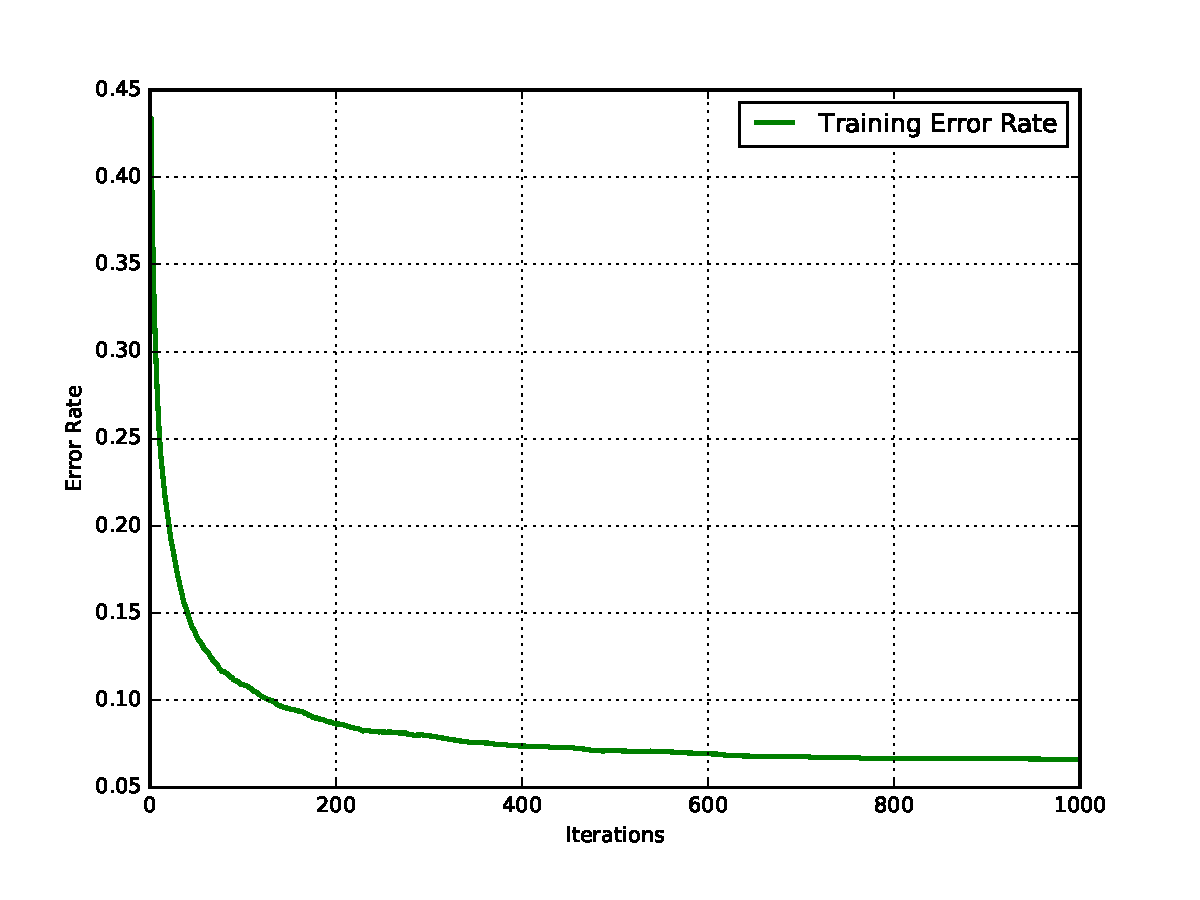
\includegraphics[width=1.0\textwidth]{./figures/tensorflow.pdf}
\caption{\label{fig:tensorflow} Result of TensorFlow (the learning rate is 0.15)}
\end{figure}

Choosing the learning rate to be 0.15, finally, after the program converges, we can calculate the training corpus error rate and evaluation corpus error rate as shown in Table \ref{table:tensorflow-error}.

\begin{table}[H]
	\centering
	\caption{\label{table:tensorflow-error} Comparison of error rate for TensorFlow}
	\begin{tabular}{c | c}
		\hline \hline
		Corpus  			&	Error rate \\[0.1cm]
		\hline
		Training corpus		&	6.66\%	\\[0.1cm]
		Evaluation corpus	&	3.52\%	\\[0.1cm]
		\hline	
	\end{tabular}\\
\end{table}


%\begin{figure}[H]
%\centering
%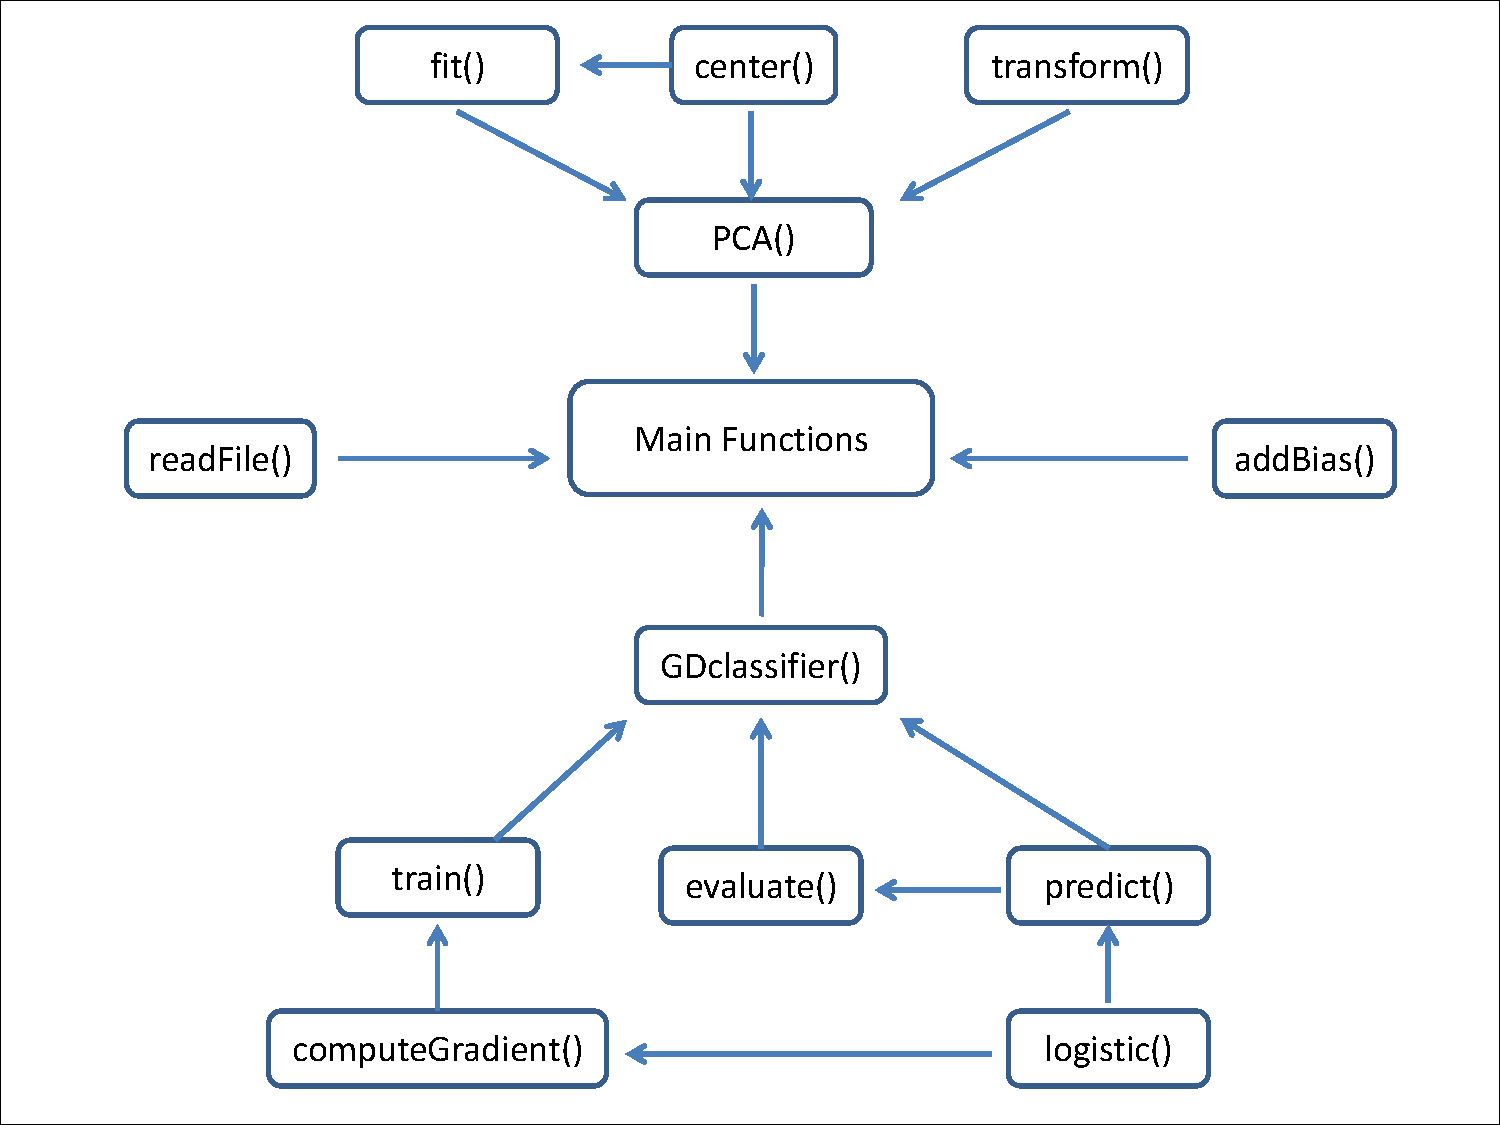
\includegraphics[width=1.0\textwidth]{./figures/diagram.pdf}
%\caption{\label{fig:diagram} Function Dependency Diagram}
%\end{figure}


%\begin{figure}[H]
%\centering
%\includegraphics[width=1.0\textwidth]{./images/detector}
%\caption{\label{fig:detector_system} Single detector system}
%\end{figure}


\clearpage

%\bibliographystyle{plain}
%\bibliographystyle{unsrt}
%\bibliography{reference.bib}

\end{document}

